\section{Introduction}
The idea of quantum computation was first proposed by Richard Feynman in 1981 to simulate quantum systems that are too hard to simulate using conventional classical digital computers.

In 1994, Peter Shor found an efficient quantum algorithm for factoring large numbers, which caused great intrest in quantum computation for its implications for cryptanalysis.

Then, it was again Peter Shor who found quantum error-correcting codes and fault-tolerant methods for executing a quantum computation reliably using noisy hardware. It makes it possible for quantum computing to be scaled up to large devices that solve very hard problems in principal.

We often use NISQ to describe the current state of quantum computation. It stands for \textit{Noisy Intermediate-Scale Quantum}. "Intermediate-Scale" conveys that today's device with more than 50 well-controlled qubits cannot be simulated by brute force using the most powerful currently existing classical computer.
"noisy" means it is still not error corrected, which limits its computational power.



Although physical realization of universal quantum computation is still in a primitive stage, there has been a lot of work in software field like IBM's QisKit, Google's Cirq and Microsoft's Q$\sharp$.
They provide software tools to describe and simulate quantum algorithms and give access of cloud quantum processors or simulators to wide community.

There are three main models of quantum computing: \textit{Quantum Turing Machine}, \textit{Quantum $\lambda$-Calculus} and \textit{Quantum Circuit}, among which the third one is the most practical.
Most quantum programming languages are \textit{quantum-circuit description languages}, which means they are used to describe the architecture of quantum circuits.
The current quantum programming languages can be categorized into two categories according to their styles: functional quantum programming languages and imperative quantum programming languages.
\begin{multicols}{2}
  \begin{center}
    Functional:
  \end{center}
  \begin{itemize}
    \item Qwire
    \item QML
    \item Quipper
    \item QuaFL
    \item Silq
  \end{itemize}

  \columnbreak

  \begin{center}
    Imperative:
  \end{center}
  \begin{itemize}
    \item QASM
    \item QCL
    \item ScaffCC
    \item Qiskit
    \item Quil
  \end{itemize}
\end{multicols}

Advanced quantum programming languages can use more powerful abstract constructs and type systems to make it easier for programmers to write correct quantum programs.
In particular, we design a simple quantum programming language named $\lambda_Q$, which means \textbf{$\boldsymbol{\lambda}$-calculus with quantum circuit}.
Its syntax consists of a traditional part, which is a simple $\lambda$-calculus, and a quantum part, whose syntax is based on Qwire~\cite{qwire}, a functional quantum programming language with linear type system.
What's more, we implement a compiler from $\lambda_Q$ to QASM (Quantum Assembly Language) ~\cite{qasm}, an imperative quantum programming language with low-level instruction sets.
The output QASM program can run on the IBM cloud quantum machine.

The main feature of $\lambda_Q$ is that the syntax for traditional computation and quantum computation are separated.
They communicate with each other via some specific operations : quantum circuit can be \textit{abstracted} or \textit{lifted (measured)} into traditional term, and traditional term for quantum circuit can be applied to quantum bits.
Thus, the syntax of quantum circuit can use \textit{linear type system} to guarantee that the Quantum Non-cloning Theorem is not violated, meanwhile the $\lambda$-calculus of the traditional part makes it easier to write quantum programs.
We will explain it in detail in Section \ref{spec}.

The overall structure of the compiler can be visualized in Figure \ref{compiler}.
The frontend is implemented using \texttt{Haskell}, and the backend is implemented using \texttt{C}.
The code can be found in \url{https://github.com/thwfhk/lambdaQ}.
We will discuss the implementation of $\lambda_Q$ compiler in detail in Section \ref{front} and \ref{back}.


\begin{center}
  \begin{figure}
    \label{compiler}
    \centering
    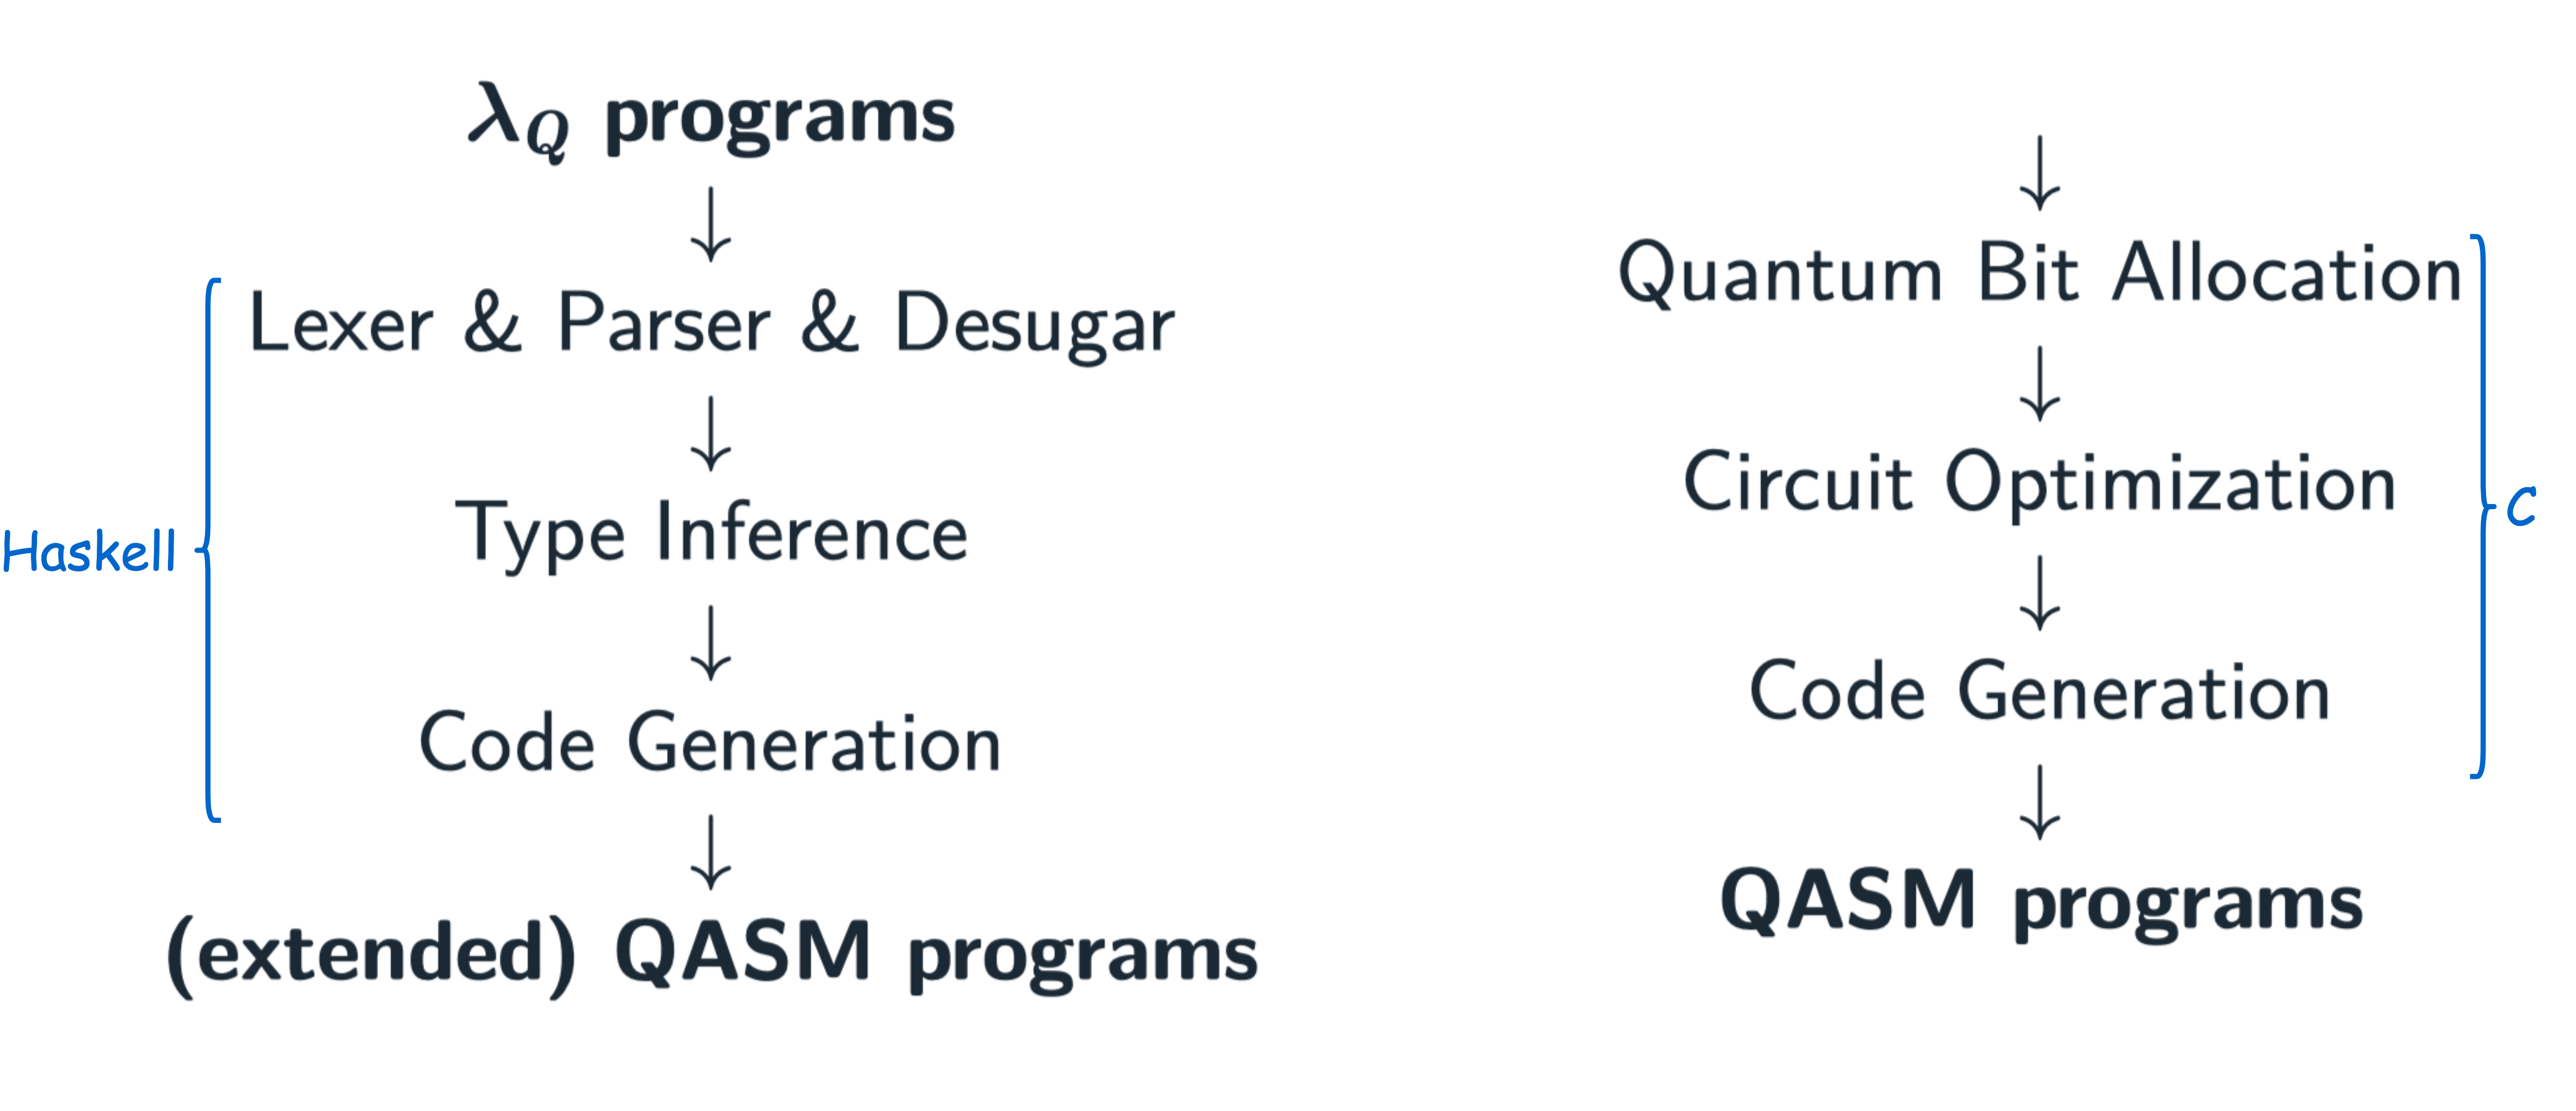
\includegraphics[width=0.9\linewidth]{images/overview.png}
    \caption{Structure of $\lambda_Q$ compiler.}
  \end{figure}
\end{center}